\documentclass[professionalfont]{beamer}
\usepackage{babel}
\usepackage{hyperref}
\usepackage[utf8]{inputenc}
\usepackage[T1]{fontenc}
\usepackage{tikz}
\usepackage{graphicx}
\usepackage{stmaryrd}
\usepackage{xcolor}
\usepackage{proof}
\usepackage{simplebnf}
\usepackage{listings}
\usepackage{amsmath}
\usetheme{material}

\usetikzlibrary{
    arrows,
    positioning,
    shapes,
    quotes
}
\newcommand{\nodes}[1]{%
    \foreach \num [count=\n starting from 0] in {#1}{
      \node[minimum size=3mm, draw, circle,fill=black!10] (n\n) at (\n,0) {\textbf{\num}};
    }
}
\lstset{language=C++,
        basicstyle={\scriptsize\ttfamily},
        keywordstyle=\color{blue}\ttfamily,
        stringstyle=\color{red}\ttfamily,
        commentstyle=\color{green}\ttfamily,
        morecomment=[l][\color{magenta}]{\#}
        }
\AtBeginSection[ ]
{
\begin{frame}{Outline}
    \tableofcontents[currentsection, hideallsubsections]
\end{frame}
}
\title{Separation Logic}
\author{Niccolò Piazzesi}
\institute[UniPi]{
    Università degli studi di Pisa \\
    Anno Accademico 2021-22
}
\begin{document}
    \begin{frame}
        \maketitle
    \end{frame}
    \begin{frame}{Outline}
        \tableofcontents[hideallsubsections]
    \end{frame}
    \section{Introduction}
    \begin{frame}
            \frametitle{Brief recap: reasoning about code}
            
            \begin{itemize}
                \item Program semantics described by logical conditions satisfied by language constructs
                \item Classical model, first put forward by Robert W. Floyd and Tony Hoare
            \end{itemize}
            
        
    \end{frame}
    \begin{frame}
        \frametitle{Floyd-Hoare Logic in 1 slide}
        \begin{center}
            \huge
            \{P\}S\{Q\}
        \end{center}
        \begin{itemize}
            \item P : pre-conditions
            \item S : statement
            \item Q : post conditions
        \end{itemize}
        \bigskip
        
        Partial correctness: \textbf{If the inital state fullfils pre-conditions and the statement terminates}, the final state satisfies the post conditions.
        \medskip

        Total correctness: \textbf{If the initial state fullfils the pre-conditions} then the statement terminates and the final state satisfies the post-conditions.
    \end{frame}

    \begin{frame}
        \frametitle{Limitations}
        
        Does not work for non terminating programs 
        \pause    
        \bigskip
        
        Becomes complex with modular constructs such as objects and unconditional jumps
        \pause
        \bigskip

        \textbf{Global view of state becomes a burden when introducing pointers( think of pointer aliasing..)}

        
    \end{frame}
\begin{frame}[fragile]
    \frametitle{Motivating example}
        \begin{columns}
    \begin{column}{0.7\textwidth}
    \begin{lstlisting}
void deletetree(struct node *root){
    if(root != NULL){
    struct node *left = root->l;
    struct node *right = root->r;
    deletetree(left);
    deletetree(right);
    free(root);
    }
}
    \end{lstlisting}
        \end{column}
            \begin{column}{0.3\textwidth}
                How can we prove memory safety?
            \end{column}
        \end{columns}
    \end{frame}
    \begin{frame}
        \frametitle{First attempt}

        
    \end{frame}
    \section{Theoretical Foundations}
    \subsection{The model and assertion language}
    \begin{frame}
        \frametitle{The model}
        \begin{columns}
            \begin{column}[]{.5\textwidth}
                Ints $\triangleq \{\cdots, -1, 0 , 1, \cdots\}$
                
                \bigskip
                Atoms, Locations $\subseteq  Ints$
                
                \bigskip
                Stores $\triangleq$ Variables  $\rightharpoonup_{fin}$ Ints
                
            \end{column}
            \begin{column}[]{.5\textwidth}
                Variables $\triangleq \{x,y,\cdots\}$

                \bigskip
                Locations $\cap $ Atoms  = \{\}, nil $\in$ Atoms

                \bigskip
                Heaps $\triangleq$ Locations $\rightharpoonup_{fin}$ Ints
            \end{column}
        \end{columns}
        
        \bigskip
        \begin{center}
        States $\triangleq$ Stores $\times$ Heaps 
        
        \bigskip
        $\llbracket E \rrbracket_s \in Ints$, $\llbracket B \rrbracket_s \in \{\text{true, false}\}$
        
        \bigskip
        $ h \in Heaps$, $h[E] \in Ints$
        \end{center}

    \end{frame}
    \begin{frame}
        \frametitle{The language}
        
        Expressions:
        \begin{equation*}
            \begin{split}
            E,F,&G := x,y,\cdots\ |\ 0\ |\ 1\ |\ E + F\ |\ E \times F\ |\ E - F \\
            &B := false\ |\ B \Rightarrow B\ |\ E=F\ |\ E<F\ |\ isatom?(E)\ | isloc?(E)
            \end{split}
        \end{equation*}
    \pause
    Assertions:
     \begin{equation*}
        \begin{split}
        P,Q,R ::&= B\ |\ E \mapsto F \hspace{21mm}Atomic\ Formulae \\
            &|\ false\ |\ P \Rightarrow Q\ |\ \forall x.P \hspace{7mm}Classical\ Logic \\
            &|\ emp\  |\ P * Q\ |\ P\ {-*}\ Q \quad Spatial\ Connectives
        \end{split}      
     \end{equation*}
     
     \begin{columns}
         \begin{column}{.5\textwidth}
             \pause
             $\neg P = P \Rightarrow False$
             
             
             $true = \neg(false)$
             
             
             $P \vee Q = \neg(P) \Rightarrow Q$  
         \end{column}
         \begin{column}{.5\textwidth}
             \pause
             $P \wedge Q = \neg(\neg P \vee \neg Q)$

             $\exists x.P = \neg\forall x.\neg P$
         \end{column}
     \end{columns}
    \end{frame}
    \begin{frame}
        \frametitle{Some notation}
        \begin{enumerate}
            \item $dom(h)$ and $dom(s)$ denote the domain of definition
            for $h \in Heaps$ and $s \in Stores$, respectively
            \bigskip
            \item $h\#h' \rightarrow dom(h) \cap dom(h') = \emptyset$
            \bigskip
            \item $ h \ast h'$ is the union of disjoint heaps
            \bigskip
            \item $(f | i \mapsto j)$ represent the partial function that behaves like $f$ except that $i$ goes to $j$.
        \end{enumerate}

        \bigskip
        $E \mapsto F_0,\cdots,F_n \triangleq (E \mapsto F_0) \ast \cdots \ast (E+n \mapsto F_n)$
        
        \medskip
        $E \doteq F \triangleq (E=F) \wedge emp$

        \medskip
        $ E \mapsto - \triangleq \exists y.E\mapsto y$
    \end{frame}
    \begin{frame}
        \frametitle{Semantics}
        
        For store $s$ and heap $h$
        \scriptsize
        \begin{card}
        \pause
        $s,h \models B\ iff\ \llbracket B \rrbracket_s = true$
       

        \bigskip
        $s,h \models  E \mapsto F\ iff\ \{\llbracket E \rrbracket_s\} = dom(h)\ and\ h(\llbracket E \rrbracket_s)=\llbracket F \rrbracket_s$
        
        
        \bigskip
        $s,h \models false \quad never $
   
        
        \bigskip
        $s,h \models  P \Rightarrow Q\ iff\ if\ s,h \models P\ then\ s,h \models Q$
        
        
        \bigskip
        $s,h \models  \forall x.P\ iff\ \forall v \in Ints. [s\ |\ x \mapsto v ],h \models P $
        \pause
        
        \bigskip
        $s,h \models  emp\ iff\ h=[]\ is\ the\ empty\ heap $
      
        \bigskip
        $s,h \models  P \ast Q\ iff\ \exists h_0, h_1. h_0 \# h_1,\ h_0 \ast h_1 = h,\ s,h_0 \models P\ and\ s,h_1 \models Q $
        
        \bigskip
        $s,h \models  P\ {-*}\ Q\ iff\ \forall h'.\ if\ h'\#h\ and\ s,h' \models P\ then\ s,h\ast h' \models Q$
       
        
        \end{card}
    \end{frame}
    \begin{frame}
        \frametitle{Visual example}
        \begin{figure}
        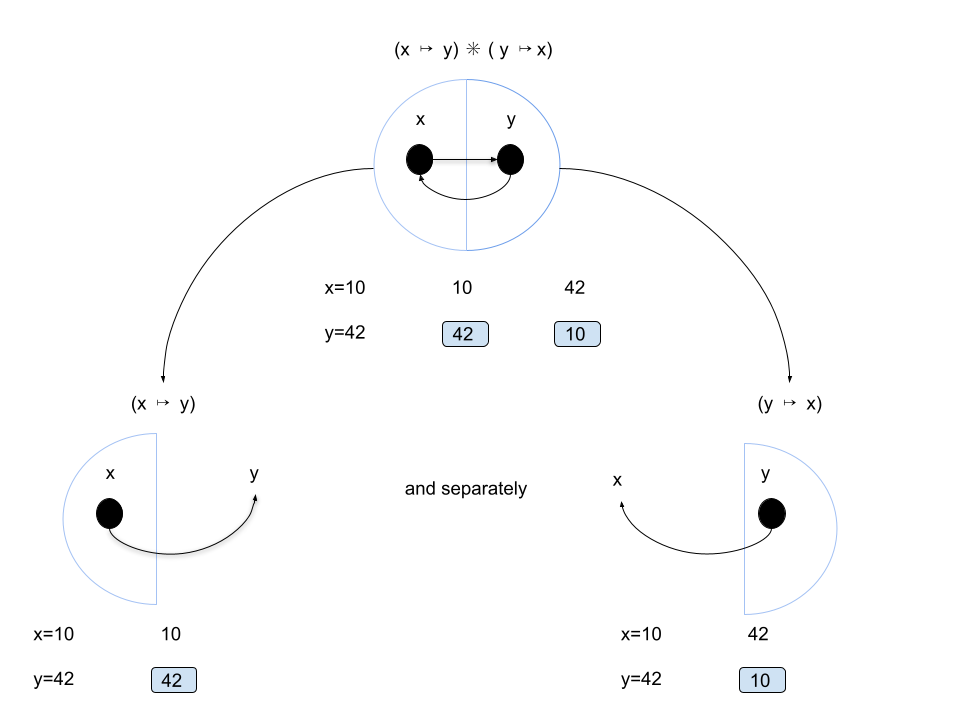
\includegraphics[width=0.9\textwidth]{img/ex1.png}
        \end{figure}
       

    \end{frame}
    \subsection{SL proofs}
        \begin{frame}
            \frametitle{Core system}
            Proof rules in seapartion logic  are divide in:\begin{enumerate}
                \item Axioms for basic mutation commands $\rightarrow$ \emph{Small axioms}
                \item Inference rules for modular reasoing $\rightarrow$ \emph{Structural rules}
            \end{enumerate}
        \end{frame}
        \begin{frame}
            \frametitle{Small axioms}
             
            \pause
            $\{E \mapsto - \}\mathbf{[E] := F}\{ E \mapsto F \} $ ("Store")
            
            \bigskip
            \pause
            $ \{E \mapsto -\} \mathbf{free(E)} \{emp\}$ ("Reclaim memory")
           
            \bigskip
            \pause 
            $ \{x\doteq m \}\mathbf{x:=cons(E_1,\cdots,E_k)} \{x \mapsto E_1[m/x],\cdots, E_k[m/x]\}$ ("Allocate memory")
            
            \bigskip
            \pause 
            $ \{x \doteq n\}\mathbf{x := E} \{ x \doteq (E[n/x])\}$ 
            
            \bigskip
            \pause 
            $ \{E \mapsto n \wedge  x = m\}\mathbf{x:=[E]} \{x=n \wedge E[m/x] \mapsto n\}$  ("Load")
    
           
        \end{frame}
        \begin{frame}
            \frametitle{Structural rules}
            \scriptsize
            \textbf{Frame Rule}
            $$
            \infer[Mod(C) \cap  Free(frame) = \emptyset]
            {\{P \ast \textcolor{red}{frame}\}C\{Q \ast \textcolor{red}{frame}\}}
            {\{P\}C\{Q\}}$$

            \pause
            \textbf{Auxiliary variable elimination}
            $$
            \infer[x \notin Free(C)]
            {\{\exists x.P\}C\{\exists x.Q\}}
            {\{P\}C\{Q\} }
            $$
        \end{frame}
        \begin{frame}
            \frametitle{Structural rules}
            \scriptsize
           \textbf{Variable substitution}
           $$
           \infer[]
           {(\{P\}C\{Q\})[E_1 / x_1, \cdots E_k /x_k] }
           {\{P\}C\{Q\} }$$
           $$
           x_i\ free\ and\ if\ x_i \in Mod(C)\ then\ E_i\ is\ not\ free\ in\ any\ E_j$$
           
           \pause
           \textbf{Rule of consequence}
            $$
            \infer[]
            {\{P\}C\{Q'\}}
            {P \Rightarrow P' \quad \{P\}C\{Q\} \quad Q \Rightarrow Q'}$$
        
        \end{frame}
    \begin{frame}
        \frametitle{Derived laws}
        The structural rules can be used to obtain more convenient derived laws.
        
        As an example, we can simplify the rule for memory allocation by assuming $x \notin Free(E_1,\cdots,E_k)$.
        $$
        \{emp\}x:=cons(E_1,\cdots, E_k)\{x \mapsto E_1,\cdots,E_k\}
        $$
        \pause

        \bigskip

        The core system can also be extended with the usual Hoare rules
        \begin{columns}
            \begin{column}{.5\textwidth}
                $$
                \infer[]{\{P\}if\ B\ then\ C\ else\ C'\{Q\}}{\{P \wedge B \}C\{Q\} \quad  \{P \wedge \neg B\}C\{Q\}}
                $$
            \end{column}
        \end{columns}
    \end{frame}
    \subsection{Examples}
    \begin{frame}[fragile]
        \frametitle{Revisiting the tree example}
        \scriptsize
    \begin{lstlisting}
void deletetree(struct node *root){
    if(root != NULL){
    struct node *left = root->l;
    struct node *right = root->r;
    deletetree(left);
    deletetree(right);
    free(root);
    }
}
    \end{lstlisting}
    
    \pause

    \textbf{Specification:}
    
    \bigskip
    \textcolor{blue}{\{tree(root)\}} deletetree(root) \textcolor{blue}{\{emp\}}
    
    \medskip
    \begin{flalign*}
        \text{\textcolor{red}{tree(root)}}\ =\ &if\ root==0\ then\ \textcolor{blue}{emp} && \\ 
        &else\ \textcolor{blue}{\exists xy.root \mapsto [l:x,r:y] \ast tree(x) \ast tree(y)} &&
    \end{flalign*}
   
    

    \end{frame}
    \begin{frame}
    \textbf{Proof:}
    \begin{flalign*}
        \{&\textcolor{red}{root \mapsto [l:left,r:right]} \ast \textcolor{blue}{tree(left)} \ast \textcolor{red}{tree(red)}\}&&
    \end{flalign*}
    \pause
    $deletetree(left);$
    \pause
    \begin{flalign*}
        \{&\textcolor{red}{root \mapsto [l:left,r:right]} \ast \textcolor{red}{emp} \ast \textcolor{blue}{tree(red)}\}&&
    \end{flalign*}
    \pause
    $deletetree(right);$
    \pause
    \begin{flalign*}
        \{&\textcolor{blue}{root \mapsto [l:left,r:right]} \ast \textcolor{red}{emp} \ast \textcolor{red}{emp}\}&&
    \end{flalign*}
    \pause
    $free(root);$
    \pause
    \begin{flalign*}
        \{&\textcolor{blue}{emp \ast emp \ast emp}\}&&\\
        \{&\textcolor{blue}{emp}\}&&
    \end{flalign*}
    \end{frame}
    \section{Reasoning with separation logic}
    \subsection{Abstract Interpretation: Biabduction and symbolic heap  analysis}
    \subsection{Model Checking for Symbolic-Heap Separation Logic }
    \section{Tools}
    \subsection{Smallfoot}
    \subsection{Infer}
    \subsection{SLAyer}
    \begin{frame}[allowframebreaks]
     
        \nocite{*}
        \frametitle{References}
        \bibliographystyle{unsrt}
        \bibliography{bib.bib}
    \end{frame}
\end{document}
